% Chapter 2 - Background

\glsresetall % reset the glossary to expand acronyms again
\chapter[Literature Review]{Literature Review}\label{ch:LitReview}
\index{Literature Review}

% Literature Review
This chapter assesses existing medical imaging denoising techniques, specifically focusing on their applicability to LODOX\textsuperscript{\textregistered} Statscan\textsuperscript{\textregistered} images.  It starts with a review of X-ray imaging theory, establishing a foundation to understand the unique challenges posed by LODOX\textsuperscript{\textregistered} Statscan\textsuperscript{\textregistered} system.  After that, it delves into a discussion of the specific image artifacts associated with this technology.  Finally, denoising algorithms used in Medical imaging are critically evaluated, assessing their suitability to LODOX\textsuperscript{\textregistered} Statscan\textsuperscript{\textregistered} images.


\section{X-ray Imaging Fundamentals}
\label{ch:LitReview:X-ray Imaging Fundamentals}
This section summarises the theoretical framework and principles of X-ray imaging. Understanding the core principles of X-ray imaging is fundamental to improving the X-ray imaging quality through denoising, particularly in the context of low-dose systems like LODOX\textsuperscript{\textregistered} Statscan\textsuperscript{\textregistered}. The following subsections will look into mechanisms of X-ray production, X-ray detection and image formation.

The fundamental X-ray imaging theory, including X-ray generation, interaction with matter, and image formation, is extensively covered in \cite{haidekker_introduction_2013},\cite{haidekker_x-ray_2013},\cite{haidekker_trends_2013}, providing a solid foundation for the subsequent discussion.



\subsection{X-ray Production}
\label{ch:LitReview:X-ray Production}
X-rays are generated in an X-ray tube by accelerating high kinetic energy electrons from the cathode across the electrostatic field in the vacuum towards the anode, striking the anode emitting X-rays. 

X-ray emission is primarily controlled by the anode voltage, which dictates the maximum energy of the X-ray photons, and the tube current, which determines the photon flux. These parameters directly influence image quality by affecting the photon count detected by the X-ray detectors. Additionally, the focal spot size of the X-ray tube plays a crucial role in image resolution as it determines the size of the X-ray beam. For instance, when the image details to be captured are smaller than the X-ray beam diameter, geometric blur is observed, which degrades image quality.

X-ray production is only one part of the imaging process; once generated, these Xrays must travel through various tissues, where their attenuation plays a critical role in the resulting image quality.






\subsection{X-ray Attenuation}
\label{ch:LitReview:X-ray Attenuation}
X-ray attenuation across various bodies is what brings about X-ray contrast. X-ray attenuation occurs when the X-ray photons collide with other atoms and get deflected from their path whilst losing some energy. The major forms of X-ray attenuation are Rayleigh Scattering, Compton Scattering, Photoelectric effect and pair production. These are summarised in the Table  \ref{XrayAttenuation} below:

\begin{center}
\small
\setlength{\arrayrulewidth}{1mm} % Thicker outer border
\setlength{\tabcolsep}{6pt} % Increase cell padding
\renewcommand{\arraystretch}{1.5} % Increase row height for readability



\begin{longtable}{ p{0.25\columnwidth}  p{0.25\columnwidth}  p{0.4\columnwidth} }

	%\hline
	\rowcolor[HTML]{D3D3D3}
	\textbf{Interaction} & \textbf{Photon Energy Range} & \textbf{Significance in Medical Imaging} \\
	%\hline
	\rowcolor[HTML]{FFFFFF} 
	Rayleigh Scattering & Low Photon Energies & Negligible Above 50 keV thus negligible influence on image quality \\
	%\hline
	\rowcolor[HTML]{F3F3F3} 
	Compton Scattering & All Photon Energies & Characteristic radiation leading to scattering that causes haze in the images. \\
	%\hline
	\rowcolor[HTML]{FFFFFF} 
	Photoelectric Effect & 50-70 keV & Crucial for X-ray contrast, especially at lower energies \\
	%\hline
	\rowcolor[HTML]{F3F3F3} 
	Pair Production & Above 1.02 MeV & Limited relevance in medical imaging as rarely seen in practice \\
	%\hline
	
	\caption{Summary of Photon Interaction Mechanisms and Their Significance in Medical Imaging.}
	\label{XrayAttenuation}

\end{longtable}
\end{center}

 In  LODOX\textsuperscript{\textregistered} Statscan\textsuperscript{\textregistered}, scattering is not an issue due to the unique detector architecture that reduces scattering by up to 95\%\cite{amirlak_novel_2009}. As X-rays are attenuated as they pass through different tissues, this varying absorption information must be recorded to generate X-ray images. The following subsection will look into the X-ray detection and image formation mechanism and how it affects the image quality.

\begin{comment}
    \begin{table}[h!]
\centering

\begin{tabular}{| p{0.25\columnwidth} | p{0.25\columnwidth} | p{0.45\columnwidth} |}
\hline

\textbf{Interaction} & \textbf{Photon Energy Range} & \textbf{Significance in Medical Imaging} \\
\hline
Rayleigh Scattering & Low Photon Energies & Negligible Above 50 keV thus negligible influence on image quality \\
\hline
Compton Scattering & All Photon Energies & Characteristic radiation leading to scattering that causes haze in the images. \\
\hline
Photoelectric Effect & 50-70 keV & Crucial for X-ray contrast, especially at lower energies \\
\hline
Pair Production & Above 1.02 MeV & Limited relevance in medical imaging as rarely seen in practice \\
\hline

\end{tabular}
\caption{Summary of Photon Interaction Mechanisms and Their Significance in Medical Imaging.}
\label{XrayAttenuation}

\end{table}
\end{comment}





\subsection{X-ray Detection and Image Formation}
\label{ch:LitReview:X-ray Detection and Image Formation}
This subsection delves into how X-ray photons are converted and detected for imaging. X-ray intensity is primarily measured using photographic films and digital detectors, necessitating conversion to another energy form, usually visible light or \gls{UV}  photons. Digital detectors are predominantly used today, as older photographic films and fluoroscope detectors were phased out due to their very low quantum efficiency and sensitivity. 

During the conversion process, these digital detectors introduce various noise components, including electronic noise and quantum noise due to the use of \gls{ASIC}. In addition, converting X-ray photons into electrical signals can introduce image artifacts such as detector blur. Detector blur occurs due to the conversion layer, which typically emits visible light in all directions. A thick conversion layer increases the likelihood of cross-talk between neighbouring pixels, while a thinner conversion layer reduces this effect and lowers quantum efficiency. Keeping the conversion layer close to the detector element can help mitigate detector blur.

Motion blur is another significant factor impacting image quality, which arises when the patient moves during exposure due to breathing. High detector sensitivity and a high photon flux from the X-ray source can allow for shorter exposure times, which reduces the likelihood of motion blur affecting the final image.




\section{Noise in X-ray imaging}
\label{ch:LitReview:Noise in X-ray imaging}
This section will examine the various types of noise inherent in X-ray imaging, specifically low-dose X-ray imaging systems such as the LODOX\textsuperscript{\textregistered} Statscan\textsuperscript{\textregistered}. It then proceeds to discuss the sources of these noises in the LODOX\textsuperscript{\textregistered} Statscan\textsuperscript{\textregistered} and concludes with an analysis of the impact of the noise on image quality and diagnosis. 


\subsection{Types of Noise in X-ray Imaging}
\label{ch:LitReview:Types of Noise in X-ray Imaging}
Noise is defined as random unwanted stochastic fluctuations and variations in brightness and colour information in an image \cite{veldkamp_dose_2009}, \cite{lahmiri_iterative_2017}. In X-ray, there are various noise types, each with a different statistical model arising from multiple sources such as the detectors' inherent properties, X-ray source, inspected objects and controller circuits \cite{seibert_tradeoffs_2004}, \cite{noauthor_noise_nodate}. The primary noise present in X-rays is Quantum noise. Other prominent noise types include Electronic and Anatomical noise. These three noise types are discussed below:


\textbf{Quantum Noise}\\
Studies show that quantum noise is predominant in \gls{PCD} \cite{noauthor_noise_nodate}, \cite{huda_radiographic_2015}. Given that \gls{PCD} are the detectors currently being used in the LODOX\textsuperscript{\textregistered} Statscan\textsuperscript{\textregistered} it is paramount to understand quantum noise. Quantum noise results primarily from X-ray photon detection and conversion \cite{kim_measurements_2024}, \cite{seibert_tradeoffs_2004}. It is produced due to the random accumulation and distribution of the X-ray photons on the detectors’ surface \cite{noauthor_noise_nodate}, \cite{veldkamp_dose_2009}, \cite{manson_image_2019}, \cite{chandra_analysis_2020}, \cite{juneja_denoising_2024}. This is shown in the Figure \ref{PoissonGen} below:
\begin{figure}[h!]
    \centering
    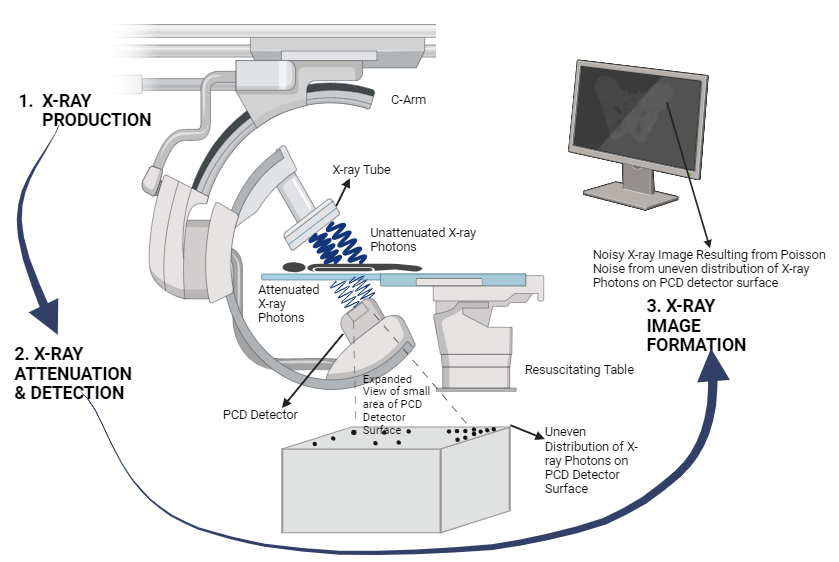
\includegraphics[width=0.5\linewidth]{3_Chapters//2_Chapter_LiteratureReview//Figures/PoissonNoise Prodcution.png}
    \caption{Diagram illustrating the generation of quantum noise in X-ray imaging due to the uneven distribution of X-ray photons on the PCD detector surface, resulting in a noisy image output. Created with \href{https://www.biorender.com}{BioRender.com}  }
    \label{PoissonGen}
\end{figure}

Due to the wide spectrum energy of X-ray photons and the randomness mentioned above, quantum noise is modelled using the Poison distribution as shown below:
\begin{equation}
P(x) = e^{-\lambda t} \frac{(\lambda t)^k}{x!}
\label{eq:poisson}
\end{equation}
Where:
\begin{table}[h!]
    %\centering
    \begin{tabular}{cc}
         P(x):& probability of distribution of photons \\
         $\lambda$:& Expected number of photons \\
         X :& measured number of photons\\
         t :& given time interval\\
    \end{tabular}
    
\end{table}

Equation \ref{eq:poisson}  depicts the signal-dependent nature of quantum noise, indicating it is not an additive noise like \gls{AWGN} as shown in studies  \cite{khan_new_2016}, \cite{thanh_review_2019}, \cite{chandra_analysis_2020}. Since quantum noise follows Poisson distribution, the expected photon count (E(x)) is equal to the variance of the photon count(var(x)) over the given time interval in Equation \ref{eq:poisson}. Thus quantum noise is proportional to the square root of the number of photons captured by the detector \cite{chandra_analysis_2020} and the square root of radiation exposure \cite{huda_radiographic_2015} as shown in equations \ref{eq:numphotons} and \ref{eq:radexposure} below:

\begin{equation}
\begin{aligned}
    E[x] &= \text{var}[x] = \lambda t \\
    \text{std}[x] &= \sqrt{\lambda t}
\end{aligned}
\label{eq:numphotons}
\end{equation}


\begin{equation}
    \sqrt{exposure level}
    \label{eq:radexposure}
\end{equation}

From the above, it can be deduced that by increasing the X-ray radiation and exposure time, quantum noise can be reduced \cite{chandra_analysis_2020}; however, this is not a suitable method in the LODOX\textsuperscript{\textregistered} Statscan\textsuperscript{\textregistered} system as it is inherently a low-dose X-ray system. 


\textbf{Electronic Noise} \\
Electronic noise typically arises from random signals caused by thermal fluctuations in interconnected electronics \cite{gravel_method_2004}, amplifier noise \cite{goyal_noise_2018}, and imperfections in detectors, such as thickness variations, scratches, and dust on the detector substrate \cite{seibert_tradeoffs_2004}. Additionally, voltage variations over the long signal distances in large detectors contribute to this noise \cite{kim_measurements_2024}. This type of noise is prevalent in \gls{CCD} \cite{gravel_method_2004} and is most pronounced at lower X-ray energy levels \cite{veldkamp_dose_2009}.

Electronic noise is modelled using the Gaussian distribution as shown in Equation \ref{eq:gaussian} as it emanates from random signals \cite{juneja_denoising_2024}:

\begin{equation}
G(x) = \left( \frac{1}{\sigma \sqrt{2\pi}} \right) e^{-\frac{(x - \mu)^2}{2\sigma^2}}
\label{eq:gaussian}
\end{equation}
Where:
\begin{table}[h!]
    %\centering
    \begin{tabular}{cc}
         $\sigma$:& represents the standard deviation \\
         X :& represents the value of the pixel \\
         $\mu$ :& represents the mean \\
    \end{tabular}
    
\end{table}

Since the LODOX\textsuperscript{\textregistered} Statscan\textsuperscript{\textregistered} now uses \gls{PCD} instead of \gls{CCD}, the impact of electronic noise is significantly reduced, with the primary source being the low X-ray doses used.


\textbf{Anatomical Noise} \\
Anatomical noise is caused by the projection of the 3D object of interest to a 2D plane, resulting in the overlapping of anatomical objects in the region of interest in the image \cite{veldkamp_dose_2009}, \cite{seibert_tradeoffs_2004}. This overlap leads to local and global camouflaging that obstructs critical parts of the image \cite{seibert_tradeoffs_2004}
. Studies have shown that anatomical noise is particularly prevalent at very low X-ray energy levels \cite{veldkamp_dose_2009}. Notably, anatomical noise is one of the most challenging to correct and affects all X-ray systems \cite{seibert_tradeoffs_2004}.

\begin{comment}
In addition to the three primary noise sources in X-ray systems discussed above, Table \ref{tab:secnoisesources} summarises less impactful secondary noise sources that primarily affect the Contrast to Noise Ratio.


\begin{table}[h!]
\tiny
\centering

\begin{tabular}{|  p{0.25\columnwidth} |  p{0.75\columnwidth} |}
\hline
\textbf{Secondary Noise Source} & \textbf{Description} \\
\hline
\textbf{Swank Noise} & Results from the variation in light output as a function of absorption depth in a scintillator, adding to the overall noise. \\
\hline
\textbf{Spatial Sampling and Quantization Errors} & Occur during the conversion of a continuous analogue signal into a discrete digital signal. \\
\hline
\textbf{Scatter} & If an antiscatter grid is used, grid cutoff or grid lines can inject unwanted noise into the image. \\
\hline
\textbf{Errors in Flat Fielding Correction} & Flat fielding is used to reduce noise caused by stationary detector non-uniformities. It works by acquiring a uniformly exposed, low-noise image (or series of images) to identify and correct variations by applying a normalized and inverted correction image. \\
\hline
\textbf{Aliasing} & A distortion that occurs when a high-frequency signal is undersampled, leading to artifacts in the image. \\
\hline

\end{tabular}
\caption{Table: Secondary Noise Sources Affecting Contrast to Noise Ratio in X-ray Systems}
\label{tab:secnoisesources}
\end{table}

\end{comment}

 

\subsection{Impact of Noise on Image Quality and Diagnosis}
\label{ch:LitReviewImpact of Noise on Image Quality and Diagnosis}

Noise in X-ray systems significantly impacts image quality, particularly at low doses \cite{veldkamp_dose_2009}. It can introduce obstructions that render images non-diagnostic \cite{manson_image_2019}. Additionally, it can introduce artifacts that hinder the acquisition of quality images, potentially leading to false diagnoses\cite{goyal_noise_2018}. Moreover, degradation in image quality makes visual interpretation difficult\cite{warner_understanding_2020}, \cite{lahmiri_iterative_2017}
, complicating diagnostics for medical professionals \cite{khan_new_2016}. Finally, the corruption of X-ray images due to noise further impairs diagnostic accuracy\cite{chandra_analysis_2020},\cite{umadevi_improved_2011}
,\cite{dong_x-ray_2020} ultimately hindering effective clinical decision-making.


\section{Denoising}
From section \ref{ch:LitReviewImpact of Noise on Image Quality and Diagnosis}, it has been established that noise degrades the image quality, thus making denoising a critical part of the pre-processing chain. The primary objective of denoising is to effectively suppress noise while preserving the image integrity \cite{juneja_denoising_2024},  \cite{lahmiri_iterative_2017}, \cite{kumar_noise_2017}. Broadly, there are three X-ray denoising methods, as shown below:

\begin{enumerate}
    \item \textbf{Use of customised hardware:} Done through incorporating hardware filters such as Aluminium filters in the X-ray machines to help reduce noise \cite{lee_impact_2022}.
    \item \textbf{Increase in X-ray dose:} An increase in the X-ray dose used significantly reduces the noise in the image. However, the dose is hindered by the Maximum Permissible Dose(MPD); thus, the dose cannot be arbitrarily increased \cite{kirti_poisson_2017}.
    \item \textbf{Digital Denoising Algorithms:} Involves using digital image processing algorithms to reduce the noise digitally.
\end{enumerate}

Digital denoising algorithms are widely used as they are not as expensive as hardware customisation and do not increase radiation risk to the patients as the increasing X-ray dose method, thus making it the most effective technique to consider for denoising LODOX\textsuperscript{\textregistered} Statscan\textsuperscript{\textregistered} images. 

The type of noise in the images significantly impacts the effectiveness of denoising algorithms, and studies caution against the assumption that all noise is \gls{AWGN} \cite{kirti_poisson_2017}. As highlighted in Section \ref{ch:LitReview:Types of Noise in X-ray Imaging}, quantum noise is the most common in X-ray images, especially in low-dose settings. Consequently, noise-independent denoising algorithms do not work well on X-ray images, making Poisson-based methods the preferred approach \cite{thanh_review_2019}, \cite{kipele_poisson_2023}. Studies have suggested two approaches to handle Poisson noise, as discussed below:

\begin{enumerate}
    \item \textbf{Poisson Direct Denoising methods}: Model the Poisson noise statistics, which are usually helpful when the images suffer from very high noise levels \cite{kirti_poisson_2017}, \cite{kipele_poisson_2023}.
    \item \textbf{Poisson \gls{VST} Denoising methods:} Involves transforming the Poisson noise to Gaussian noise because when the photon count is large enough, Poisson distribution approaches Gaussian, and the \gls{Anscombe transform} is used to stabilising the variance of the Poisson noise \cite{kipele_poisson_2023}.
\end{enumerate}

However, denoising X-ray images presents several critical challenges discussed below:

\begin{enumerate}
    \item \textbf{Maintaining flat regions:} Flat regions in the image must remain flat without introducing noise or artifacts \cite{juneja_denoising_2024}.
    \item \textbf{Preserving image boundaries:} Image boundaries must be retained without causing blurring \cite{juneja_denoising_2024}.
    \item \textbf{Protecting global contrast and textural features:} The global contrast should be preserved, and textural details should not be lost [19].
    \item \textbf{Avoiding new artifacts:} The denoising process should not generate any new artifacts in the image \cite{juneja_denoising_2024}, \cite{thanh_review_2019}.
\end{enumerate}
 
 
Over the years, various algorithms have been proposed to address these four challenges. These algorithms are generally classified into three broad categories: Classical Filters, Hybrid Filters and Deep learning methods \cite{juneja_denoising_2024}, \cite{kirti_poisson_2017}. The following section will analyse each category in detail, exploring their advantages, disadvantages, and suitability for handling Poisson noise in the LODOX\textsuperscript{\textregistered} Statscan\textsuperscript{\textregistered}.

\subsection{Classical Filters}
This subsection briefly discusses the classical \gls{DSP} filters implemented to combat noise in X-ray Images, broadly classified into spatial and transform filters.  Spatial filters are further categorised into linear and non-linear filters. Linear filters are easy to implement as they apply non-discriminate denoising to all the pixels without prior categorisation \cite{khan_new_2016} and thus are not good with signal-dependent noise leading to artifacts and blurring \cite{juneja_denoising_2024}, \cite{mandic_denoising_2018}. In contrast, non-linear filters first detect noisy pixels and then replace them selectively, making them more effective for denoising \cite{khan_new_2016}.

\textbf{Spatial Domain Filters} \\
This subsection discusses key spatial domain filters currently used for X-ray image denoising. A detailed analysis of these filters, outlining their strengths, weaknesses, and applicability to LODOX\textsuperscript{\textregistered} Statscan\textsuperscript{\textregistered} images, is discussed below. 

\gls{ADF} is a spatial diffusion filter that adaptively smooths images, preserving important anatomical structures by controlling diffusion across edges \cite{chandra_analysis_2020}
. Although \gls{ADF} effectively preserves micro-texture and edges, its performance degrades with larger mask sizes, reducing its ability to handle quantum noise \cite{chandra_analysis_2020}
. Additionally, \gls{ADF} is slow, and its effectiveness depends heavily on careful parameter selection, and when not done correctly it tends to remove some image details degrading image quality \cite{juneja_denoising_2024}, \cite{chandra_analysis_2020}
. Consequently, this makes \gls{ADF} less suitable for the high levels of quantum noise in LODOX\textsuperscript{\textregistered} Statscan\textsuperscript{\textregistered} images.

Despite \gls{ADF}'s ability to maintain micro-texture and edges, its shortcomings in dealing with quantum noise in LODOX\textsuperscript{\textregistered} Statscan\textsuperscript{\textregistered} images make exploring alternative techniques, such as the \gls{BF}, necessary. \gls{BF} is a non-iterative filter that merges grey levels of pixels based on their spatial and photometric similarity, preserving sharp structural patterns while suppressing noise \cite{juneja_denoising_2024}, \cite{chandra_analysis_2020}. However, \gls{BF} is prone to gradient reversal artifacts near edges, leading to a loss of fine detail \cite{juneja_denoising_2024}, \cite{chandra_analysis_2020}. Kirti et al. \cite{thanh_review_2019},\cite{thakur_poisson_2016} attempted to address this by developing an enhanced version, \gls{PRBF}, adding the capability to remove Poisson Noise, although it still struggles with photon-limited images. Given that LODOX\textsuperscript{\textregistered} Statscan\textsuperscript{\textregistered} images are photon-limited, the \gls{BF} may not be ideal for denoising.

Since \gls{BF} struggles with photon-limited images, exploring other filters that can effectively handle quantum noise, such as \gls{TV} filters, is necessary. \gls{TV} filter popularly known as \gls{ROF} was first developed by Rudin et al. \cite{rudin_nonlinear_1992} and is an edge-preserving algorithm designed to handle discontinuities in anatomical details \cite{khan_new_2016}, \cite{rodrigues_denoising_2008}. Studies show that \gls{TV} is effective in denoising Poisson and Gaussian noise \cite{rodrigues_denoising_2008}; however, it struggles to preserve edges, produces the \gls{Staircase effect} \cite{rodrigues_denoising_2008} and has long processing times \cite{lee_x-ray_2018}. Over time researchers have sought to address these challenges by improving the initial version of the \gls{TV} algorithm.  Some of these adaptions are summarised in Table \ref{tab:TV} below:

\begin{center}
\small
\setlength{\arrayrulewidth}{1mm} % Thicker outer border
\setlength{\tabcolsep}{6pt} % Increase cell padding
\renewcommand{\arraystretch}{1.5} % Increase row height for readability

\begin{longtable}{ p{0.2\columnwidth}  p{0.3\columnwidth}  p{0.4\columnwidth} }
%\hline
\rowcolor[HTML]{D3D3D3} 
\textbf{Algorithm} & \textbf{Description} & \textbf{Challenges} \\
%\hline
\rowcolor[HTML]{FFFFFF} 
\gls{R-L} and \gls{TV} (Dey et al.) \cite{dey_deconvolution_2004} & Combined \gls{R-L} and \gls{TV} to develop a Poisson-based denoising algorithm specifically suited for microscopy images. & Only Tailored for microscopy images \\
%\hline
\rowcolor[HTML]{F3F3F3} 
\gls{MROF} (Triet et al.) \cite{le_variational_2007} & An improved version of \gls{ROF} that can process Poisson noise. & Long execution times, Artificial artifacts, Cannot handle photon-limited images. \\
%\hline
\rowcolor[HTML]{FFFFFF} 
\gls{ATV} (Prasath) \cite{prasath_quantum_2017} & Developed to address artificial artifacts in \gls{MROF}. & Faces the same challenges as \gls{MROF}. \\
%\hline
\rowcolor[HTML]{F3F3F3} 
Enhanced \gls{ATV} (Liu et al.) \cite{liu_poisson_2017} & Modified \gls{ATV} to denoise photon-limited images. & Long execution times. \\
%\hline
\caption{Summary of Adaptations to \gls{TV} Filters to addressing challenges in original \gls{TV} filter.}
\label{tab:TV}

\end{longtable}
\end{center}


\begin{comment}
\begin{center}
\small
\begin{longtable}{| p{0.2\columnwidth} | p{0.3\columnwidth} | p{0.4\columnwidth} |}
\hline
\textbf{Algorithm} & \textbf{Description} & \textbf{Challenges} \\
\hline
\gls{R-L} and \gls{TV} (Dey et al.)\cite{dey_deconvolution_2004} & Combined \gls{R-L} and \gls{TV} to develop a Poisson-based denoising algorithm specifically suited for microscopy images. & 
Only Tailored for microscopy images
 \\
\hline
\gls{MROF}(Triet et al.)\cite{le_variational_2007} & An improved version of \gls{ROF} that can process Poisson noise. & 


    Long execution times,
    Artificial artifacts,
    Cannot handle photon-limited images.

 \\
\hline
\gls{ATV} (Prasath)\cite{prasath_quantum_2017} & Developed to address artificial artifacts in \gls{MROF}. & 
Faces the same challenges as \gls{MROF}.
 \\
\hline
Enhanced \gls{ATV} (Liu et al.) \cite{liu_poisson_2017} & Modified \gls{ATV} to denoise photon-limited images. & 
Long execution times.
 \\
\hline
\caption{Summary of Adaptations to \gls{TV} Filters to addressing  challenges in original \gls{TV} filter.}
\label{tab:TV}


\end{longtable}

\end{center}

 \gls{NLM} has emerged as an alternative to denoise photon-limited images to address the shortcomings of \gls{TV} filters. \gls{NLM} uses a non-local averaging technique that operates on all similar pixels, removing noise after exploring redundant information \cite{juneja_denoising_2024}, \cite{khan_new_2016}, \cite{rodrigues_denoising_2008}. Consequently, this leads to high detail preservation in images \cite{rodrigues_denoising_2008}. However, despite the high detail preservation, \gls{NLM} suffers from slow execution time due to the computational overhead arising from the complexity of evaluating the pixel weights \cite{juneja_denoising_2024},\cite{rodrigues_denoising_2008}. Various researchers have proposed solutions to address the challenges, as summarised in Table \ref{tab:NLM} below:



\begin{center}
\small

\begin{longtable}{| p{0.2\columnwidth} | p{0.3\columnwidth} | p{0.4\columnwidth} |}
\hline
\textbf{Researcher(s)} & \textbf{Proposed Solution} & \textbf{Challenges Addressed} \\
\hline
Mahmoudi and Sapiro\cite{1542113} & Modified \gls{NLM} by adding Pre-selection of neighborhoods & Increased speed \\
\hline
Pierrick Coupe \cite{coupe_fast_2006} & Added parallel processing & Improved execution time \\
\hline
Deledalle et al. \cite{5653394} & Modified \gls{NLM} to incorporate Poisson noise statistics & Tailored for Poisson noise \\
\hline
Shim et al.\cite{shim_feasibility_2018} & Implemented \gls{FNLM} & Significant speed improvement i.e 3.7 times faster than \gls{TV} filter \\
\hline
Lee et al. \cite{lee_impact_2022} & Combined \gls{NLM} denoising algorithm with Aluminium additive hardware filters & Superior results in \gls{CNR}, \gls{COV}, \gls{NIQE}, and \gls{BRISQUE} \\
\hline
Lee \cite{lee_x-ray_2018} & \gls{FNLM} with acceleration function and Euclidean distance & Superior \gls{NNPS}, \gls{CNR}, and \gls{COV} values; fast processing time (0.17s) \\
\hline

\caption{Summary of Proposed Solutions to Address Challenges in \gls{NLM} Filter}
\label{tab:NLM}
\end{longtable}

\end{center}

\end{comment}

 \gls{NLM} has emerged as an alternative to denoise photon-limited images to address the shortcomings of \gls{TV} filters. \gls{NLM} uses a non-local averaging technique that operates on all similar pixels, removing noise after exploring redundant information \cite{juneja_denoising_2024}, \cite{khan_new_2016}, \cite{rodrigues_denoising_2008}. Consequently, this leads to high detail preservation in images \cite{rodrigues_denoising_2008}. However, despite the high detail preservation, \gls{NLM} suffers from slow execution time due to the computational overhead arising from the complexity of evaluating the pixel weights \cite{juneja_denoising_2024},\cite{rodrigues_denoising_2008}. Various researchers have proposed solutions to address the challenges, as summarised in Table \ref{tab:NLM} below:


\begin{center}
\small
\setlength{\arrayrulewidth}{1mm} % Thicker outer border
\setlength{\tabcolsep}{6pt} % Increase cell padding
\renewcommand{\arraystretch}{1.5} % Increase row height for readability

\begin{longtable}{ p{0.2\columnwidth}  p{0.3\columnwidth}  p{0.4\columnwidth} }
%\hline
\rowcolor[HTML]{D3D3D3} 
\textbf{Researcher(s)} & \textbf{Proposed Solution} & \textbf{Challenges Addressed} \\
%\hline
\rowcolor[HTML]{FFFFFF} 
Mahmoudi and Sapiro \cite{1542113} & Modified \gls{NLM} by adding Pre-selection of neighborhoods & Increased speed \\
%\hline
\rowcolor[HTML]{F3F3F3} 
Pierrick Coupe \cite{coupe_fast_2006} & Added parallel processing & Improved execution time \\
%\hline
\rowcolor[HTML]{FFFFFF} 
Deledalle et al. \cite{5653394} & Modified \gls{NLM} to incorporate Poisson noise statistics & Tailored for Poisson noise \\
%\hline
\rowcolor[HTML]{F3F3F3} 
Shim et al. \cite{shim_feasibility_2018} & Implemented \gls{FNLM} & Significant speed improvement i.e 3.7 times faster than \gls{TV} filter \\
%\hline
\rowcolor[HTML]{FFFFFF} 
Lee et al. \cite{lee_impact_2022} & Combined \gls{NLM} denoising algorithm with Aluminium additive hardware filters & Superior results in \gls{CNR}, \gls{COV}, \gls{NIQE}, and \gls{BRISQUE} \\
%\hline
\rowcolor[HTML]{F3F3F3} 
Lee \cite{lee_x-ray_2018} & \gls{FNLM} with acceleration function and Euclidean distance & Superior \gls{NNPS}, \gls{CNR}, and \gls{COV} values; fast processing time (0.17s) \\
%\hline
\caption{Summary of Proposed Solutions to Address Challenges in \gls{NLM} Filter}
\label{tab:NLM}

\end{longtable}
\end{center}

%\newpage
\gls{NLM} filters still suffer from slow execution due to computational complexity and require high-speed hardware to execute faster, thus limiting their suitability for denoising LODOX\textsuperscript{\textregistered} Statscan\textsuperscript{\textregistered} images. 

%\newpage
\textbf{Transform Domain Filters} \\
This subsection details some transform domain filters used in X-ray image denoising. Unlike spatial filters, transform domain filters operate by converting the image into an alternative representation, such as the Wavelet or Fourier domain, where denoising is performed, after which the image is transformed back to the spatial domain using an inverse transform. A detailed analysis of these filters, outlining their strengths, weaknesses, and applicability to LODOX\textsuperscript{\textregistered} Statscan\textsuperscript{\textregistered} images, is discussed below. 

Gaussian filter is the most widely used transform domain filter known for reducing edge blurring and computational efficiency; however, it loses a lot of image detail \cite{juneja_denoising_2024}
, \cite{khan_new_2016}. Given that Gaussian filter works is tailored for Gaussian noise, it struggles to denoise Poisson noise prevalent in LODOX\textsuperscript{\textregistered} Statscan\textsuperscript{\textregistered}. Researchers have opted for other transform domain filters to denoise X-ray images to address these shortcomings. 

One of the filters that has shown promise in improving the shortcomings of the Gaussian filter is the wiener filter. It is an \gls{MSE}-optimal stationary filter that balances noise smoothing and inverse filtering, using local image variance for adaptive smoothing \cite{juneja_denoising_2024}, \cite{chandra_analysis_2020}, \cite{noauthor_wiener_nodate}. Studies have shown that the wiener filter effectively reduces Gaussian impulse and speckle noise whilst preserving the edges \cite{chandra_analysis_2020}, \cite{wang_noise_2008}.  However, despite these advantages, it only provides a point estimate that gives optimal results under specific conditions, making it less effective in handling signal-dependent noises such as Poisson \cite{juneja_denoising_2024}. Additionally, it leads to blurry images due to the use of fixed kernel size \cite{chandra_analysis_2020}.

Researchers have attempted to improve the Wiener filter to enhance its performance. For instance, Goreke \cite{goreke_novel_2023} modified a wiener filter by incorporating an \gls{FIR} filter with \gls{ASO} optimisation, demonstrating its superiority over \gls{NLM}, \gls{BF}, \gls{BM3D}, \gls{PURE-LET}, Bayes, and \gls{DTCWT} filters in terms of contrast index, entropy, sharpness, and computational efficiency. Additionally, Lahmiri \cite{lahmiri_iterative_2017} developed a multistep iterative Wiener filter where the denoised output from one step is the input to the next stage, stopping based on an energy condition and showed that it could denoise and restore the original texture in finite iterations. However, this approach was limited to Gaussian noise\cite{lahmiri_iterative_2017}, reducing its applicability to other noise types. Despite these improvements, the Wiener filter still struggles to handle Poisson noise, making it a less suitable option for LODOX\textsuperscript{\textregistered} Statscan\textsuperscript{\textregistered} images, which are predominantly degraded by Poisson noise.

While the wiener filter preserves the image texture,  its limitations in handling quantum noise suggest that complementary methods, such as wavelet filters, are necessary for optimal denoising. Primarily, wavelet filters operate by applying shrinkage or thresholding to wavelet coefficients, followed by image synthesis \cite{rodrigues_denoising_2008}.  The local definition of features allows wavelet filters to preserve minute edges and details in X-ray images \cite{juneja_denoising_2024}, \cite{rodrigues_denoising_2008}.  Notably, wavelet filters are associated with challenges of estimating an appropriate threshold and the tendency to introduce artifacts leading to smooth edges at times \cite{juneja_denoising_2024}, \cite{rodrigues_denoising_2008}. To address these challenges associated with the wavelet filter, researchers have developed various variations, which are summarised in Table \ref{tab:wavelet} below:

%Resing ahs to be done later, maybe consider using long table format

\begin{comment}
    \begin{center}
\small
%\fontsize{7}{8}\selectfont
\begin{longtable}{| p{0.2\columnwidth} | p{0.3\columnwidth}  | p{0.2\columnwidth} | p{0.2\columnwidth} |}

\hline
\textbf{Researcher(s)} & \textbf{Method} \& \textbf{Description} & \textbf{Strengths} & \textbf{Limitations} \\
\hline
Thierry et al.  \cite{LUISIER2010415} & \gls{PURE-LET}:Based on the unnormalised Haar wavelet transform, the minimisation of unbiased \gls{MSE} estimate & Handles Poisson noise

Competitive in denoising and computational complexity & Cannot handle photon-limited images \\
\hline
Timmermann and Nowak \cite{761328} & \gls{MMI} Model:A simple Bayesian intensity estimate procedure & Denoises photon-limited images & Highly complex \\
\hline
Zhang et al. \cite{4531116} & \gls{MS-VST}: Extension of \gls{Anscombe transform} combining wavelet, ridgelet, and curvelet & Denoises photon-limited images & Highly complex \\

\hline
Wang \cite{wang_noise_2008} & Adaptive Wavelet Wiener Filter: Pre-processing, three-wavelet decomposition using Daubechies wavelet (db5),  \gls{IBS} & Superior performance in preserving edges, enhancing image quality in low-dose X-ray and medical images & Highly complex \\
\hline
Kaur et al.\cite{1273218} & Wavelet-Based Statistical: Uses realistic distribution of wavelet coefficients & Better feature preservation in medical images & Highly complex \\
\hline
Du et al. \cite{6568145} & \gls{DTCWT}: Dual-tree complex wavelet transform & Better than wavelet transform filters in Poisson noise reduction in X-ray images & Highly complex \\
\hline
\caption{Summary of Wavelet Filter Variations for Poisson Noise Reduction in Medical and X-ray Images, Highlighting Strengths and Challenges}
\label{tab:wavelet}

\end{longtable}
\end{center}
\end{comment}

\begin{center}
\small
\setlength{\arrayrulewidth}{1mm} % Thicker outer border
\setlength{\tabcolsep}{6pt} % Increase cell padding
\renewcommand{\arraystretch}{1.5} % Increase row height for readability

\begin{longtable}{ p{0.15\columnwidth}  p{0.3\columnwidth}   p{0.2\columnwidth}  p{0.2\columnwidth} }

%\hline
\rowcolor[HTML]{D3D3D3} 
\textbf{Researcher(s)} & \textbf{Method} \& \textbf{Description} & \textbf{Strengths} & \textbf{Limitations} \\
%\hline
\rowcolor[HTML]{FFFFFF} 
Thierry et al.  \cite{LUISIER2010415} & \gls{PURE-LET}: Based on the unnormalised Haar wavelet transform, the minimisation of unbiased \gls{MSE} estimate & Handles Poisson noise. Competitive in denoising and computational complexity & Cannot handle photon-limited images \\
%\hline
\rowcolor[HTML]{F3F3F3} 
Timmermann and Nowak \cite{761328} & \gls{MMI} Model: A simple Bayesian intensity estimate procedure & Denoises photon-limited images & Highly complex \\
%\hline
\rowcolor[HTML]{FFFFFF} 
Zhang et al. \cite{4531116} & \gls{MS-VST}: Extension of \gls{Anscombe transform} combining wavelet, ridgelet, and curvelet & Denoises photon-limited images & Highly complex \\
%\hline
\rowcolor[HTML]{F3F3F3} 
Wang \cite{wang_noise_2008} & Adaptive Wavelet Wiener Filter: Pre-processing, three-wavelet decomposition using Daubechies wavelet (db5),  \gls{IBS} & Superior performance in preserving edges, enhancing image quality in low-dose X-ray and medical images & Highly complex \\
%\hline
\rowcolor[HTML]{FFFFFF} 
Kaur et al. \cite{1273218} & Wavelet-Based Statistical: Uses realistic distribution of wavelet coefficients & Better feature preservation in medical images & Highly complex \\
%\hline
\rowcolor[HTML]{F3F3F3} 
Du et al. \cite{6568145} & \gls{DTCWT}: Dual-tree complex wavelet transform & Better than wavelet transform filters in Poisson noise reduction in X-ray images & Highly complex \\
%\hline
\caption{Summary of Wavelet Filter Variations for Poisson Noise Reduction in Medical and X-ray Images, Highlighting Strengths and Challenges}
\label{tab:wavelet}
\end{longtable}
\end{center}


 
The wavelet filter has proven effective in denoising photon-limited images by preserving fine edges and details while reducing Poisson noise. Despite challenges such as determining the optimal threshold and potential edge smoothing, advanced variations like \gls{IBS} techniques have enhanced its performance. These methods, particularly when using Daubechies wavelet (db5), demonstrate superior capability in handling low-dose X-ray images, making wavelet filters a potential denoiser for  LODOX\textsuperscript{\textregistered} Statscan\textsuperscript{\textregistered}  images.

\subsection{Hybrid Filters}
Hybrid filters have gained popularity for X-ray image denoising due to the non-adaptability of classical filters, as they are suited to handling specific types of noises. Hybrid filters include filters that combine two or more classical filters or use entirely non-classical spatial and transform methods to denoise the images. This subsection summarises the most notable hybrid filter approaches, strengths, and limitations.

One of the most successful hybrid filters is 3D transform domain filtering.  These methods convert 2D images into 3D domain and apply a sliding window to process the blocks, matching similar regions to effectively reduce noise through shrinking coefficients in the 3D arrays \cite{rodrigues_denoising_2008}. The most widely used 3D domain filter is the \gls{BM3D}, which is known for its significant noise reduction while preserving local texture information \cite{chandra_analysis_2020}. However, \gls{BM3D} faces challenges when the image is heavily contaminated with noise, leading to overshooting, which can obscure the structural information in X-ray images \cite{chandra_analysis_2020}.

Over time, researchers have developed various \gls{BM3D} modifications to address the abovementioned challenges.  For instance,  Makitalo et al. \cite{6212354} modified the \gls{BM3D} for Poisson noise by incorporating an \gls{Anscombe transform} to stabilise the variance of Poisson-corrupted images. Additionally, Harrison et al. \cite{harrison_multichannel_2017} developed a custom version of \gls{BM3D} specifically for \gls{PCCT} scanners called \gls{BM3D}\textunderscore \gls{PCCT} that uses four energy thresholds and exploits correlation and exact alignment between energy bins to denoise the images.  They demonstrated that \gls{BM3D}\textunderscore \gls{PCCT} achieved a 65.0\% reduction in noise standard deviation, tighter clustering of attenuation values, and smaller mean angular differences compared to \gls{BM3D} \cite{harrison_multichannel_2017}. Ren \cite{ren_simulation_2023} also developed a denoising method based on subspace decomposition, employing sparse representation and block matching to suppress noise. In simulations using a three-dimensional digital mouse phantom, Ren’s method improved the peak signal-to-noise ratio by 2.21 dB compared to existing techniques when the photon flux was  $4 \times 10^3$ \cite{ren_simulation_2023}.

Although \gls{BM3D} is the most widely used hybrid filter, several other filters have been developed to address its shortcomings. However, most of these alternatives are not widely adopted. Table \ref{tab:hybrid} below summarises these filters.


\begin{comment}
\begin{center}
\small

\begin{longtable}{|  p{0.2\columnwidth} |  p{0.2\columnwidth} |  p{0.2\columnwidth} |  p{0.25\columnwidth} |}
\hline
\textbf{Researcher} & \textbf{Hybrid Filter Method} & \textbf{Advantages} & \textbf{Limitations} \\
\hline
Salmon et al. \cite{salmon2014poisson} & Non-local \gls{PCA} & Better noise reduction compared to \gls{BM3D} & Increased execution time due to iterative nature; struggles with noise detection in high-dimensional data. \\
\hline
Kipele \cite{kipele_poisson_2023} & \gls{PCA} combined with \gls{NLM} & Performs well in reducing noise in images with moderate intensity & Performance not tested for extreme Poisson noise levels. \\
\hline
Wensen et al. \cite{doi:10.1137/16M1072930} & \gls{HNIPM} trained on \gls{Anscombe transform} & Removes Poisson noise in both high and low-peak images & Long execution time; not suitable for photon-limited images. \\
\hline
Jisha \& Suresh \cite{jisha2014poisson} & \gls{Anscombe transform} with Curvelet and \gls{MS-VST} & Performs better than most wavelet-based filters & Execution time may be high; tested on specific noise types. \\
\hline
Dong \cite{dong_x-ray_2020} & Wavelet filter combined with median filter & Preserves image details while reducing noise & Tested only on Gaussian and Salt-and-Pepper noise; efficacy on Poisson noise not verified. \\
\hline
Dabov et al. \cite{4271520} & Non-local adaptive nonparametric filtering & Similar performance to \gls{NLM} and \gls{Yaroslavsky filter} & Limited testing on medical X-ray images; complex computational process. \\
\hline
He et al. \cite{6319316} & Guided filter & Superior performance compared to bilateral filter; reduces quantum noise & Dependent on parameter selection and guidance image; large filter masks lead to blurring. \\
\hline
Treece et al. \cite{7559744} & Bitonic filter & Effectively reduces noise without artifacts; good edge preservation & Can cause significant blurring if not carefully applied. \\
\hline
Mandic et al. \cite{mandic_denoising_2018} & \gls{LPA-RICI} adaptive algorithm & Less execution time due to easy parallelisation & Limited testing on specific noise types. \\
\hline
Umadevi et al. \cite{umadevi_improved_2011} & Bi-orthogonal Haar wavelets with BayesShrink thresholding and \gls{ICA} & Achieves high-quality images quickly (PSNR = 44.85) & May not work as efficiently in photon-limited settings. \\
\hline
Kirti \cite{kirti_poisson_2017} & Hybrid filter combining non-local means and \gls{BM3D} collaborative filtering & Encouraging results with Poisson noise; improved PSNR over wavelet-based methods & Execution time still an issue compared to faster filters. \\
\hline

\caption{Summary of Hybrid Filters for X-ray Image Denoising}
\label{tab:hybrid}
\end{longtable}

\end{center}
\end{comment}

\begin{center}
\small
\setlength{\arrayrulewidth}{1mm} % Thicker outer border
\setlength{\tabcolsep}{6pt} % Increase cell padding
\renewcommand{\arraystretch}{1.5} % Increase row height for readability

\begin{longtable}{ p{0.2\columnwidth}  p{0.2\columnwidth}  p{0.2\columnwidth}  p{0.25\columnwidth} }
%\hline
\rowcolor[HTML]{D3D3D3} 
\textbf{Researcher} & \textbf{Hybrid Filter Method} & \textbf{Advantages} & \textbf{Limitations} \\
%\hline
\rowcolor[HTML]{FFFFFF} 
Salmon et al. \cite{salmon2014poisson} & Non-local \gls{PCA} & Better noise reduction compared to \gls{BM3D} & Increased execution time due to iterative nature; struggles with noise detection in high-dimensional data. \\
%\hline
\rowcolor[HTML]{F3F3F3} 
Kipele \cite{kipele_poisson_2023} & \gls{PCA} combined with \gls{NLM} & Performs well in reducing noise in images with moderate intensity & Performance not tested for extreme Poisson noise levels. \\
%\hline
\rowcolor[HTML]{FFFFFF} 
Wensen et al. \cite{doi:10.1137/16M1072930} & \gls{HNIPM} trained on \gls{Anscombe transform} & Removes Poisson noise in both high and low-peak images & Long execution time; not suitable for photon-limited images. \\
%\hline
\rowcolor[HTML]{F3F3F3} 
Jisha \& Suresh \cite{jisha2014poisson} & \gls{Anscombe transform} with Curvelet and \gls{MS-VST} & Performs better than most wavelet-based filters & Execution time may be high; tested on specific noise types. \\
%\hline
\rowcolor[HTML]{FFFFFF} 
Dong \cite{dong_x-ray_2020} & Wavelet filter combined with median filter & Preserves image details while reducing noise & Tested only on Gaussian and Salt-and-Pepper noise; efficacy on Poisson noise not verified. \\
%\hline
\rowcolor[HTML]{F3F3F3} 
Dabov et al. \cite{4271520} & Non-local adaptive nonparametric filtering & Similar performance to \gls{NLM} and \gls{Yaroslavsky filter} & Limited testing on medical X-ray images; complex computational process. \\
%\hline
\rowcolor[HTML]{FFFFFF} 
He et al. \cite{6319316} & Guided filter & Superior performance compared to bilateral filter; reduces quantum noise & Dependent on parameter selection and guidance image; large filter masks lead to blurring. \\
%\hline
\rowcolor[HTML]{F3F3F3} 
Treece et al. \cite{7559744} & Bitonic filter & Effectively reduces noise without artifacts; good edge preservation & Can cause significant blurring if not carefully applied. \\
%\hline
\rowcolor[HTML]{FFFFFF} 
Mandic et al. \cite{mandic_denoising_2018} & \gls{LPA-RICI} adaptive algorithm & Less execution time due to easy parallelisation & Limited testing on specific noise types. \\
%\hline
\rowcolor[HTML]{F3F3F3} 
Umadevi et al. \cite{umadevi_improved_2011} & Bi-orthogonal Haar wavelets with BayesShrink thresholding and \gls{ICA} & Achieves high-quality images quickly (PSNR = 44.85) & May not work as efficiently in photon-limited settings. \\
%\hline
\rowcolor[HTML]{FFFFFF} 
Kirti \cite{kirti_poisson_2017} & Hybrid filter combining non-local means and \gls{BM3D} collaborative filtering & Encouraging results with Poisson noise; improved PSNR over wavelet-based methods & Execution time still an issue compared to faster filters. \\
%\hline

\caption{Summary of Hybrid Filters for X-ray Image Denoising}
\label{tab:hybrid}
\end{longtable}

\end{center}


 
Hybrid filters have emerged as an effective solution for addressing the limitations of classical filters by combining multiple techniques to handle different types of noise. These filters, such as those based on \gls{PCA}, curvelet transforms, and adaptive models, show improved noise reduction, edge preservation, and execution efficiency. Notably, hybrid methods like adaptive wavelet Wiener preprocessing and variations of \gls{BM3D} tailored for Poisson noise have demonstrated superior performance in enhancing image quality in medical X-ray imaging, making them well-suited for the complex noise characteristics present in LODOX\textsuperscript{\textregistered} Statscan\textsuperscript{\textregistered} images.


\subsection{Deep Learning Methods}
This subsection provides a brief overview of  \gls{ML} methods applied to medical imaging denoising, highlighting their advantages and associated challenges.


Machine learning, particularly deep learning, has transformed data processing by solving complex problems, including medical image denoising. Deep learning employs artificial neural networks to learn the characteristics of a given problem and develop effective solutions. In medical image denoising, ML models are trained to identify and remove noise patterns from the images. These models fall into two broad categories: supervised learning, which requires clean, labelled data (ground truth), and unsupervised learning, which does not require ground truth data. Unsupervised learning models are preferred as in clinical settings, acquiring noise-free data in medical imaging is impractical, except through simulations, which may not always accurately reflect real-world conditions \cite{hariharan_learning-based_2019}.

The shift from conventional filters to \gls{ML} methods has been driven by several challenges. Studies have shown that the manual selection of filters is a cumbersome process requiring good domain knowledge \cite{juneja_denoising_2024}.  Additionally, many conventional filters rely on prior noise information, further complicating optimisation \cite{juneja_denoising_2024}. In contrast, ML methods require relatively few tuning parameters and learn by themselves to denoise images \cite{nadkarni_deep_2023}. For instance,  \gls{CNN} excel at extracting relevant features from noisy data and can be trained efficiently using parallel processing with \gls{GPU}s \cite{juneja_denoising_2024}. This makes \gls{ML} methods more efficient than conventional filters in many cases.

The following will explore several specific applications of deep learning frameworks that denoise X-ray images with a specific focus on unsupervised models. \gls{N2N} and \gls{N2V} are the two most common unsupervised deep learning denoising methods that have been used in medical image denoising as they do not require clean reference images, making them well-suited for applications such as LODOX\textsuperscript{\textregistered} Statscan\textsuperscript{\textregistered} image denoising.

Lehtinen et al. \cite{pmlr-v80-lehtinen18a} developed \gls{N2N}  to address the challenge of requiring clean and noisy image pairs during the model training phase. \gls{N2N} makes use of two noisy images each with an independent noise distribution to learn the underlying signal from these noise-corrupted data points. Studies have shown \gls{N2N} achieving comparable performance to models trained with clean images. For instance, Lehtinen et al. \cite{pmlr-v80-lehtinen18a} trained the \gls{N2N} for 300 epochs with noisy targets and achieved an average \gls{PSNR} of 31.10 dB on the validation set, while training with clean targets reached 31.14 dB, comparable to previous work by Wang et al. \cite{wang2016accelerating} and Lee et al. \cite{7950457}. Additionally, \gls{N2N} can generalise across various types of noise distributions \cite{pmlr-v80-lehtinen18a}. The use of noisy image pairs during training and adapting to various noise types makes \gls{N2N} a highly suitable model for denoising LODOX\textsuperscript{\textregistered} Statscan\textsuperscript{\textregistered} images where noise is prevalent and acquiring images is impossible.

Krull et al. \cite{8954066} developed \gls{N2V} to eliminate the need for paired noisy images during the training phase. \gls{N2V} uses single noisy images to train the network to predict the values of randomly masked pixels, encouraging the model to learn spatial relationships in the data. This makes \gls{N2V} highly adaptable to various noise types as minimal assumptions about the underlying noise distribution are made. Krull et al. \cite{8954066}  demonstrated \gls{N2V} applicability to various imaging modalities by running experiments on photography, fluorescence microscopy, and cryo-Transmission Electron Microscopy. They concluded that as long as the assumptions of predictable signal and pixel-wise independent noise are met, \gls{N2V} performance is comparable to traditional and \gls{N2N}-trained models \cite{8954066}. Since \gls{N2V} does not require clean images or paired noisy images, it is a highly scalable solution, well-suited for LODOX\textsuperscript{\textregistered} Statscan\textsuperscript{\textregistered} images.

Both Noise2Noise and Noise2Void are promising models for medical image denoising due to their unsupervised nature, effectively addressing the challenges of acquiring clean training data in a clinical context like Lodox imaging.

Other attempts to denoise X-ray images primarily using supervised learning are summarised in Table \ref{tab:deeplearning} below: 


\begin{comment}
\begin{center}
\small

\begin{longtable}{| p{0.2\columnwidth} | p{0.2\columnwidth} |  p{0.2\columnwidth} |  p{0.3\columnwidth} |}
\hline
\textbf{Author(s)} & \textbf{Proposed Model}  & \textbf{Strengths} & \textbf{Challenges} \\
\hline
Zhang et al. \cite{7839189} & \gls{DnCNN}: Neural network that outputs residual noise (V) and computes clean X-ray (C) as the sum of noisy observation and residual image & Outperforms \gls{BM3D} and \gls{WNNM} & Not effective for Poisson noise \\
\hline
Hariharan \cite{hariharan_learning-based_2019} & Learning-based model using model-based simulations and data-driven normalisation for robust denoising & Outperforms \gls{BM3D} and \gls{WNNM}; produces visually superior results & Limited clinical practicality due to reliance on simulated data \\
\hline
Nadkarni et al. \cite{nadkarni_deep_2023} & Custom 2-D \gls{U-Net} \gls{CNN} for quick iterative reconstruction and accurate material decomposition across energy thresholds & 15 times faster than iterative reconstruction; higher spatial resolution & Relies on supervised learning and high computational resources; training detector prone to distortions \\
\hline
Huber et al. \cite{huber_dedicated_2022} & \gls{CNN} model using \gls{U-Net} for ultra-high-resolution \gls{PCD} \gls{CT}, trained with image-based noise insertion & Retains fine details and low contrast signals; preferred by radiologists & Limited by supervised learning and high-quality training data requirements \\
\hline
Chang et al. \cite{chang_improved_2024} & \gls{PKAID-Net} using prior knowledge-aware iterative denoising neural network using lower-noise \gls{VMI} for improved denoising & 96\% noise reduction; maintains spatial and spectral fidelity & Potentially complex iterative refinement may limit practical application \\
\hline
Baffour et al. \cite{baffour_photon-counting_2023} & \gls{CNN} model for detecting multiple myeloma using \gls{PCD} \gls{CT} images & Enhanced detection of abnormalities; better clarity and accuracy & Focused on detection and denoising only a small subset \\
\hline
Durcos et al. \cite{ducros2017regularization} & Uses regularisation strategy to suppress noise & Easy to implement & Limited noise suppression effect across various noise types \\
\hline
Zhang et al. \cite{zhang2020multi} & Third-Order Tensor Model that combines \gls{TV} regularisation with tensor similarity and image sparsity & Improved noise suppression & High computational costs due to tensor reconstruction \\
\hline
Sun et al. \cite{sun_research_2024}
 & \gls{FBPtransNet} that combines \gls{U-Net} \gls{CNN} with Transformer module for improved image detail restoration & Outperforms \gls{TV} and \gls{FBPconvNet}; clearer image details & Does not clearly address Poisson noise \\
\hline

\caption{Summary of Deep Learning Approaches for X-Ray Image Denoising}
\label{tab:deeplearning}
\end{longtable}

\end{center}

\end{comment}

\begin{center}
\small
\setlength{\arrayrulewidth}{1mm} % Thicker outer border
\setlength{\tabcolsep}{6pt} % Increase cell padding
\renewcommand{\arraystretch}{1.5} % Increase row height for readability

\begin{longtable}{ p{0.2\columnwidth}  p{0.2\columnwidth}   p{0.2\columnwidth}   p{0.3\columnwidth} }
%\hline
\rowcolor[HTML]{D3D3D3} 
\textbf{Author(s)} & \textbf{Proposed Model}  & \textbf{Strengths} & \textbf{Challenges} \\
%\hline
\rowcolor[HTML]{FFFFFF} 
Zhang et al. \cite{7839189} & \gls{DnCNN}: Neural network that outputs residual noise (V) and computes clean X-ray (C) as the sum of noisy observation and residual image & Outperforms \gls{BM3D} and \gls{WNNM} & Not effective for Poisson noise \\
%\hline
\rowcolor[HTML]{F3F3F3} 
Hariharan \cite{hariharan_learning-based_2019} & Learning-based model using model-based simulations and data-driven normalisation for robust denoising & Outperforms \gls{BM3D} and \gls{WNNM}; produces visually superior results & Limited clinical practicality due to reliance on simulated data \\
%\hline
\rowcolor[HTML]{FFFFFF} 
Nadkarni et al. \cite{nadkarni_deep_2023} & Custom 2-D \gls{U-Net} \gls{CNN} for quick iterative reconstruction and accurate material decomposition across energy thresholds & 15 times faster than iterative reconstruction; higher spatial resolution & Relies on supervised learning and high computational resources; training detector prone to distortions \\
%\hline
\rowcolor[HTML]{F3F3F3} 
Huber et al. \cite{huber_dedicated_2022} & \gls{CNN} model using \gls{U-Net} for ultra-high-resolution \gls{PCD} \gls{CT}, trained with image-based noise insertion & Retains fine details and low contrast signals; preferred by radiologists & Limited by supervised learning and high-quality training data requirements \\
%\hline
\rowcolor[HTML]{FFFFFF} 
Chang et al. \cite{chang_improved_2024} & \gls{PKAID-Net} using prior knowledge-aware iterative denoising neural network using lower-noise \gls{VMI} for improved denoising & 96\% noise reduction; maintains spatial and spectral fidelity & Potentially complex iterative refinement may limit practical application \\
%\hline
\rowcolor[HTML]{F3F3F3} 
Baffour et al. \cite{baffour_photon-counting_2023} & \gls{CNN} model for detecting multiple myeloma using \gls{PCD} \gls{CT} images & Enhanced detection of abnormalities; better clarity and accuracy & Focused on detection and denoising only a small subset \\
%\hline
\rowcolor[HTML]{FFFFFF} 
Durcos et al. \cite{ducros2017regularization} & Uses regularisation strategy to suppress noise & Easy to implement & Limited noise suppression effect across various noise types \\
%\hline
\rowcolor[HTML]{F3F3F3} 
Zhang et al. \cite{zhang2020multi} & Third-Order Tensor Model that combines \gls{TV} regularisation with tensor similarity and image sparsity & Improved noise suppression & High computational costs due to tensor reconstruction \\
%\hline
\rowcolor[HTML]{FFFFFF} 
Sun et al. \cite{sun_research_2024} & \gls{FBPtransNet} that combines \gls{U-Net} \gls{CNN} with Transformer module for improved image detail restoration & Outperforms \gls{TV} and \gls{FBPconvNet}; clearer image details & Does not clearly address Poisson noise \\
%\hline

\caption{Summary of Deep Learning Approaches for X-Ray Image Denoising}
\label{tab:deeplearning}
\end{longtable}

\end{center}


\section{Conclusion}
%Will still need to be redone in a better way just a placeholder
The literature review provided a comprehensive analysis of classical and modern denoising techniques, mainly focusing on their applicability to low-dose systems such as the LODOX\textsuperscript{\textregistered} Statscan\textsuperscript{\textregistered} systems. 

The review began with a brief overview of X-ray imaging fundamentals, including X-ray production, attenuation, and detection and their significance to image quality. This was followed by an analysis of noise types in X-ray images. It was highlighted that the predominant noise degrading X-ray images is Poisson noise, and various Posison denoising methods were looked into. A plethora of classical \gls{DSP} filters was looked into, highlighting their limitations in handling photon-limited images. Despite some variations of wavelet and \gls{NLM} filters showing promise, they often fell short of effectively reducing Poisson noise without compromising image quality. The review then transitions to hybrid filters, particularly the \gls{BM3D}. \gls{BM3D} demonstrates significant improvement over classical filters but still faces challenges in denoising noise-heavy images such as LODOX\textsuperscript{\textregistered} Statscan\textsuperscript{\textregistered} images. This underscored the need for adaptable denoising methods to learn different noise patterns.

\gls{ML} methods like \gls{N2N} and \gls{N2V} offer significant potential due to their ability to operate without clean training data. This is critical for LODOX\textsuperscript{\textregistered} Statscan\textsuperscript{\textregistered} as it is impossible to obtain ground truth data. However, in most of the literature, the testing was mostly done on \gls{MRI}, \gls{CT} and microscopy images, with limited application to low-dose X-ray systems like the LODOX\textsuperscript{\textregistered} Statscan\textsuperscript{\textregistered}. While \gls{N2N} and \gls{N2V} have shown adaptability across various noise types in other imaging domains, applying these models to the LODOX\textsuperscript{\textregistered} Statscan\textsuperscript{\textregistered} system presents both a challenge and an opportunity for further research. This project aims to bridge this gap by adapting and enhancing \gls{N2N} and \gls{N2V} models specifically for LODOX\textsuperscript{\textregistered} Statscan\textsuperscript{\textregistered} images, documenting the results and challenges encountered in this process. This approach addresses the current limitations in the literature and contributes to the development of more effective denoising techniques for low-dose X-ray imaging.
